\documentclass[../main.tex]{subfiles}
\chapter{Simulation}
\label{c:simulation}

\begin{figure}
	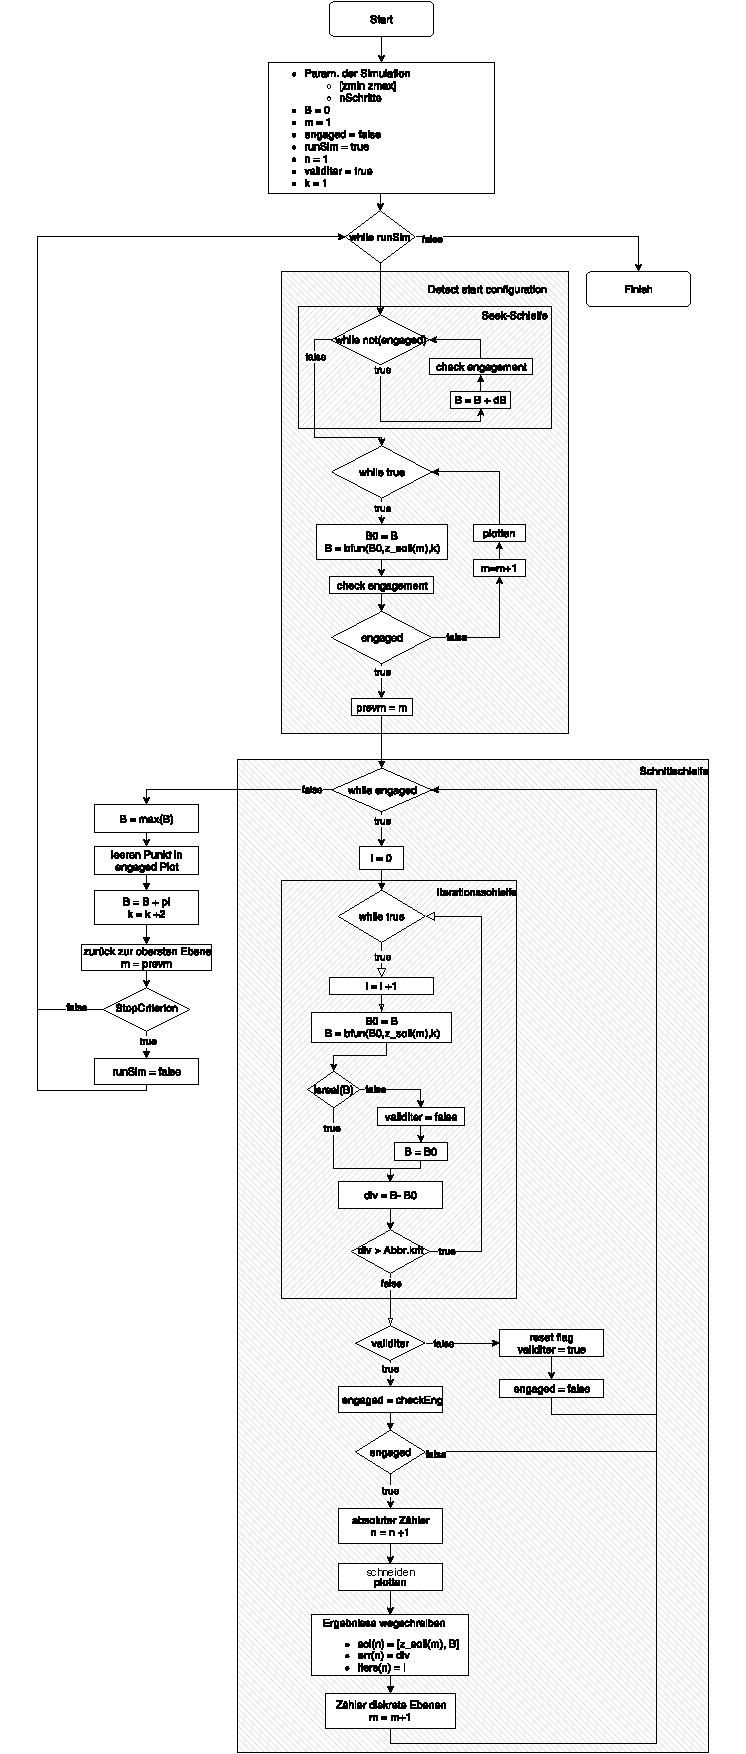
\includegraphics[scale=0.75]{vf1-flowchart}
	\caption{Hier ist die caption}
	\label{fig:flowchart}
\end{figure}

Abbildung \ref{fig:flowchart} zeigt das Flussbild der Simulation.
Der Ablauf der Simulation ist unterteilt in die Abschnitte Findung der Startkonfiguration, Durchführung der Schnitte mit den Lösungsiterationen, Erkennung des Schnittendes sowie Nachbereitung des Schnittes und schließlich Abschluss der Simulation.
Neben der Ausführung des Simulationscodes sollte der Status der Berechnung in Form von grafischen Ausgaben dargestellt werden.
Das Plotten von Daten in Echtzeit ist schwierig zu realisieren in \matlab, vor Allem bei dreidimensionalen Datensätzen.
Die standardmäßig zur Verfügung gestellten Routinen sind nicht gut optimiert für schnelle Ausführungszeit und es ist notorisch schwierig \matlab Code multithread-fähig zu gestalten.
Die Lösungsansätze um trotz dieser Herausforderungen die für die grafische Ausgabe beanspruchte Rechenzeit effizient zu nutzen und die Simulation möglichst geringfügig zu belasten wird ebenfalls besprochen.


Die einzelnen Prozessschritte der Simulation werden im Folgenden erläutert.

\section{Vorbereitung der Simulation}
Vor Beginn der Simulation wird die Simulationssteuerungsparameter eingelesen.
Dabei werden zunächst die Eingabedaten des betrachteten Falles festgelegt.
Mit folgende Parameter kann definiert werden, wie dieser Fall gestaltet ist:
\begin{itemize}
	\item Zähnezahl des Zahnrades
	\item Modul des Zahnrades
	\item Geometrie des des Werkzeuges (Durchmesser, Kopf- und Fußhöhe)	
\end{itemize}
Aus diesen Parametern können weitere Startbedingungen ermittelt werden.
So ist die Startposition des Werkzeugs und den daraus folgenden Positionen der Maschinenkomponenten zu berechnen wie sie in Abschnitt \ref{c:maschkomppos} besprochen wurden.
Die Position der X-Achse der Maschine wird berechnet über den Achsabstand des gedachten Schneckengetriebes nach \cite[Gleichung 23.4]{Matek2017}:
\begin{equation*}
	a = \frac{d_{s1}+d_{s2}}{2}
\end{equation*}
\begin{eqdscr}{$d_{s1}$, $d_{s2}$}
	\item[$a$] Achsabstand
	\item[$d_{s1}$, $d_{s2}$] Teilkreisdurchmesser von Schneckenrad und Schnecke
\end{eqdscr}
Der Teilkreisdurchmesser des Schneckenrades wird berechnet nach \cite{Matek2017}:
\begin{equation*}
	d_{s1} = m \cdot z
\end{equation*}
\begin{eqdscr}{$m$}
	\item[$m$] Modul
	\item[$z$] Zähnezahl des Werkstückes
\end{eqdscr}
Der Vorschubfaktor der X-Achse $\feed{X}{\wz}$ ist im betrachteten Fall 0, sie verändert also ihre Position ausgehend von der Startposition im Verlauf der Simulation nicht.

Für den Startwert der Y-Achse müssen die Größen $y$, Achsverschiebung im Ausgang, und $\yshift$ festgelegt werden.
Ebenso ist für den Achsvorschub der Y-Achse $\feed{Y}{\wz}$ ein Wert einzugeben.
Diese Größen sind im betrachteten Fall 0.
Die Y-Achse verändert im betrachteten Fall ihrer Position ausgehend von ihrem Startwert nicht.

Danach wird die Werkzeuggeometrie erzeugt.
Wie in Kapitel \ref{c:werkzeugkinematik} erläutert wird die Geometrie des Werkzeuges in Polarkoordinaten beschrieben.
Dabei wird im aktuellen Stand das Bezugsprofil durch vier Eckpunkte dargestellt, deren Koordinaten mit einem Algorithmus von \scherbarth berechnet werden.
Da eine Zahnstange als Zahnrad mit unendliche großer Zähnezahl verstanden werden kann, hat sie gerade Flanken \cite[Kap. 3]{Widmer1981}.
Eine Annäherung der Zahnstange mit vier Punkten ist deswegen zweckmäßig, obwohl Verrundungen am Zahnkopf damit noch nicht dargestellt werden können.

Die Simulation beginnt mit einem Ebenenindex m von 1.
Es wird davon ausgegangen, dass die erste ebene des Werkstücks geschnitten wird.
Vor jedem Schnitt wird dann die oberste Ebene ermittelt, die eine valide Schnittkonfiguration hervorbringt.
Wie diese Erkennung funktioniert wird in Abschnitt \ref{c:seeken} erläutert.

\section[Startkonfiguration]{Findung der Startkonfiguration}
\label{c:startkonfig}
Der erste Schritt zur Findung der Startkonfiguration bei jeder Werkzeugumdrehung ist die Suche nach einer Werkzeugkonfiguration bei welcher Kontakt zwischen Werkzeug und Werkstück auftritt.
Dieser Vorgang wird als Seeken, eine deutsche Form des englischen Wortes für ,,Suchen'', bezeichnet.
Dabei wird das Werkzeug im freien Raum rotiert bis Kontakt auftritt.
Im Anschluss wird dann eine validen Schnittkonfiguration gesucht.

Eine valide Schnittkonfiguration tritt auf, wenn die auf eine diskrete Ebene des Werkstücks projizierte Geometrie der Schneide Überdeckung mit der Werkstückgeometrie hat.
Bei der vorliegenden Simulation ist das Werkstück entlang seiner Ausdehnung in z-Richtung in diskrete Ebenen unterteilt, welche das Werkzeug auf der jeweiligen Höhe in $z$ schneiden.
Die dabei entstehende Verschneidungsgeometrie des Werkstücks mit der Ebene ist eine zweidimensionale Geometrie.
Diese Geometrie ist ein Polygon, welches mit der Menge diskreter Punkte beschrieben, welche die Ecken des Polygons bilden.
Die Beschreibung von Werkstück und Werkzeug als Polygone wird in Abschnitt \ref{c:schnitte} im Detail beschrieben.

Seeken geschiet in der Seek-Schleife, die auch im Flussdiagrams in Abbildung \ref{fig:flowchart} beschrieben ist.
Dabei wird der Winkel des Werkzeugs ausgehend vom seiner Startkonfiguration mit einer bedatbaren Schrittweite inkrementiert, bis ein Punkt der Werkzeugschneide in der Hüllgeometrie des Werkstücks liegt.
Befindet sich ein Punkt des Werkzeugs in Hüllgeometrie des Werkstücks ist das Werkzeug ,,engaged'', von englisch ,,eingerastet''; die Schneide befindet sich im Eingriff.

Die Hüllgeomtrie des Werkstücks entspricht der Form des Rohmaterials, also ein Zylinder mit dem Durchmesser und der Höhe des Werkstücks.
Die Lage des Werkstücks entlang der z-Achse des Bearbeitungstischkoordinatensystems ist definierbar.

Engagement wird in der Funktion \code{checkEng} durch Vergleich der Position der Schneidenecken mit der Ausdehnung des Werkstücks erkannt.
Dabei ist es geschickt die Position der Schneidenecken in Zylinkerkoordinaten zu beschreibenen.
Vergleichbar zu den deckungsgleichen kartesischen und zylindrischen Koordinatensystemen des Werkzeugs, kann auch das Werkstück in kartesischen und zylindrischen Koordinatensystemen beschrieben werden.
Dieses Zylinderkoordinatensystem ist im Ursprung des kartesischen Werkzeugkoordinatensystems aufgespannt.
Die Koordinaten eines Punktes werden dann durch einen Winkel, einen Radius und eine Höhe in z-Richtung beschrieben.

Damit ein Punkt des Werkzeugs als engaged gilt, müssen zwei Bedingungen erfüllt sein:
Zum einen muss der der Abstand des Punktes zum Ursprung kleiner als der Radius des Werkstücks sein.
Zum anderen muss der Wert seiner z-Koordinate im Interval der Ausdehung des Werkstücks liegen.
Der Winkel des Punktes spielt zur Engagementerkennung keine Rolle.
Der Abstand $d$ des Punktes zum Ursprung wird als euklidische Norm berechnet nach \cite{mwVecnorm}:
\begin{equation*}
	d = \|v\| = \sqrt{\sum_{k=1}^{N} \|v_k\|^2}
\end{equation*}
Die Funktion gibt dann als logischen Wert zurück, ob der Werkzeugpunkt engaged ist oder nicht.

Das Ziel des Findens der Startkonfiguration es, die Rotation des Werkzeuges zu finden, bei welcher das Werkzeug das Werstück gerade berührt.
Der Seek liefert einen Werkzeugwinkel, der in der Nähe dieser Konfiguration liegt.
Durch Verkleinerung der Schrittweite beim Seeken, kann die Lösungskonfiguration dieses Näherungsverfahrens näher an die tatsächliche Lösung geführt werden.
Allerdings muss die Berechnung des Engagements, also des Eingriffs der Schneide, für jeden Iterationsschritt erfolgen und sollte deswegen sehr günstig sein, also wenig Rechenzeit in Anspruch nehmen.
Gleichzeit muss ein Kompromiss zwischen der Größe der Schrittweite beim Seeken und der dafür notwendigen Rechenzeit gefunden werden.
Allerdings kann mit einem nachträglichen Schritt eine Lösungskonfiguration weit innerhalb des Werkstück-Envelopes geschickt ausgeglichen werden.

Sobald durch Iteration eine Konfiguration gefunden wurde, die als engaged gewertet wird, kann der so gefundene Winkel des Werkzeugs $B$ als Eingangswert $B_0$ für Gleichung \ref{eq:loesung} verwendet werden.
Neben dem Startwert $B_0$ sind für diese Funktion zur Lösung noch zwei Größen notwendig.

Zum einen muss die Höhe der Ebene in z für die gelöst werden soll gegeben sein.
Andererseit muss die Lösung der Funktion verschoben werden, um den bereits zurück gelegten Winkel des Werkzeugs.

Dies geschieht über den Vorfaktor $k$.
Beim ersten Schnitt des Werkzeugs ist der Vorfaktor 1, weil die Startposition des Werkzeugs auf der xz-Ebene im Koordinatensystem in Abbildung \ref{fig:hobspindle_coord} ist.
Die Lösung des Werkzeugwinkels muss im zweiten oder dritten Quadranten des Koordinatensystems liegen.
Der Lösungsbereich des Arkussinus ist $\left[-\frac{\pi}{2}, \frac{\pi}{2}\right]$.
Es muss also $1 \cdot \pi$ addiert werden um eine Lösung im dritten Quadranten, mit Wertebereich $\left[\frac{\pi}{2}, \frac{3\cdot \pi}{2}\right]$, zu erhalten.

Es ist also noch nicht bekannt, auf welcher Ebene das Werkzeug das Werkzeug initial berührt.
Auf dieser Ebene soll der Punkt des Werkzeugs, für den gelöst wird, liegen und der Wert der z-Koordinate dieser Ebene wird in Gleichung \ref{eq:loesung} als $z_{soll}$ bezeichnet.
Am Anfang der Simulation ist die geometrische Beziehung von Werkzeug und Werkstück unbekannt.
Die initiale Schnittebene kann aber geschickt durch ein iteratives Verfahren gefunden werden.
Gleichung \ref{eq:loesung} wird für einen Wert für $z_{soll}$ gelöst.
Anschließend wird für die Lösung $B$ geprüft, ob sich das Werkzeug in dieser Konfiguration engaged ist.
Ist dies nicht der Fall, wird für die Lösung die nächst tiefergelegene Ebene verwendet.
Das Werkzeug bewegt sich entlang seiner Rotation mit abfallender Höhe in z näher zur Achse des Werkstücks und kann so in Berührung kommen.
Für diese Ebene wird gelöst und wieder auf Engagement geprüft.

Zwar muss so bei den iterativen Schritten ebenfalls wiederholt Engagement geprüft.
Allerdings kann die endgültige Lösung gespeichert werden und für die nächste Werkzeugumdrehung als Startebene verwendet werden.
Es kann bei gleichbleibendem Werkstückradius und geringem Vorschub in z-Richtung davon ausgegangen werden, dass die Kontaktebene bei der nächsten Umdrehung nahe der aktuellen liegt und somit nur wenige Iterationen notwendig sind.

Nach Finden einer Werkzeugkonfiguration die zu einem validen Schnitt führt, kann mit der Simulation des Schneidevorgangs begonnen werden.

\section{Berechnung des Werkzeugwinkels}
Zu jedem Schnittvorgang ist die Berechnung des Werkzeugwinkels notwendig.

Die Eckpunkte der Schneide bewegen sich während der Rotation auf einer Kreisbahn um die Werkzeugachse.
Sie liegen dabei nicht zwangsläufig auf einer Ebene, die durch die Werkzeugachse geht oder parallel dazu ist.
Damit ist diese Schneidenebene nicht parallel zu den Schnittebenen des Werkstücks.
Das bedingt zwei grundsätzliche Probleme, die es zu lösen gilt.
Auf der einen Seite, muss die Schneide des Werkzeugs auf die Werkstückebene projiziert werden, um die Verscheidungsberechnung durchführen zu können.
Die Projektion wird in Abschnitt \ref{c:schnitte} betrachtet.
Auf der anderen Seite, gibt es für jeden Punkt der Schneide einen einzigartigen Winkel, den das Werkzeug annehmen muss, damit dieser Punkt auf einer Schnittebene des Werkstücks liegt.

Gelöst wird dieses Problem für jeden Punkt der Schneide durch Berechnung eines individuellen Winkels des Werkzeugs.
So wird jeder Werkzeugwinkel gefunden, bei denen die Punkte auf der Zielschnittebene des Werkstücks liegt.
Dafür wird Gleichung \ref{eq:loesung} iterativ gelöst.
Dabei handelt es sich um ein Fixpunktproblem.
Dem Fixpunktproblem zugrunde liegt eine Fixpunktgleichung der Form:
\begin{equation*}
	x = g(x)
\end{equation*}
Zur Lösung dieses Problems wird in \cite{Widmer1981} vorgeschlagen eine Fixpunktiteration durchzuführen.
Dabei wird in die Gleichung umgeformt, sodass sie in folgender Form vorliegt:
\begin{equation*}
	x^{\left(n+1\right)} = g(x^{\,n}), \quad n = 0{,} 1{,} \dots
\end{equation*}
\begin{eqdscr}{$k$}
	\item[$n$] Iterationsindex
\end{eqdscr}
,,Für jede Wahl des Startpunktes $x^{(0)}$ konvergiert die Folge der Iterierten gegen'' \cite{Widmer1981} gegen die Lösung des Fixpunktproblems.
Da die iterative Methode fehlerbehaftet ist, ist es notwendig ein Abbruchkriterium einzuführen.
Dabei bietet sich die Änderung der Lösung zwischen Iterationen an.
Ist diese kleiner als ein definiert Wert, wird das Verfahren abgebrochen und die finale Lösung verwendet.
Diese Methode ist im Flussbild in dem Block ,,Iterationsschleife'' realisiert.

Entsprechend der Methode wird Gleichung \ref{eq:loesung} so angepasst, dass also der rechten Seite statt $B$ die Lösung des vorhergehenden Iterationsschrittes $B_0$ verwendet wird.
\begin{equation}
	B = k \cdot \pi - \phi_\wz + \arcsin{\left(\dfrac{Z - c - z_{soll} + B_0 \cdot{} \feed{Z}{Wz} + \sin(A) \cdot{} (Y + \yshift + B_0 \cdot{} \feed{Y}{Wz} - h_\wz)}
		{r_\wz \cdot{} \cos(A)}\right)}
\end{equation}
Diese Methode hat sich als sehr geeignet und effizient erwiesen.
So sind bei einer beispielhaften Simulation nur maximal zwei Iterationsschritte notwendig gewesen um das Abbruchkriterium von $1\cdot10^{-3}$zu erreichen.

Die Methode bietet außerdem den Vorteil, dass als Startwert für die iterative Lösung des nächsten Werkszeugpunktes die letzte Lösung verwendet kann.
Das ist möglich, da bei geringem Abstand der Schnittebenen des Werkstücks auch die Lösungen nahe beieinander liegen müssen.

\section{Durchführung der Schnitte}
\label{c:schnitte}
Zu Beginn der Beschreibung der Schnittsimulation soll erklärt werden, wie in der Simulation einen Schnitt berechnet wird.
Werkzeug und Werkstück werden als Polygone repräsentiert, die in Matlab als Objekt der Klasse polyshape dargestellt werden.
Polyshape Objekte haben Methoden, die es erlauben Verschneidungsoperationen durchzuführen.
Dabei wird von einem polyshape Objekte die Geomtrie abgezogen, die von dem anderen Polygon überlagert wird.
\begin{figure}
	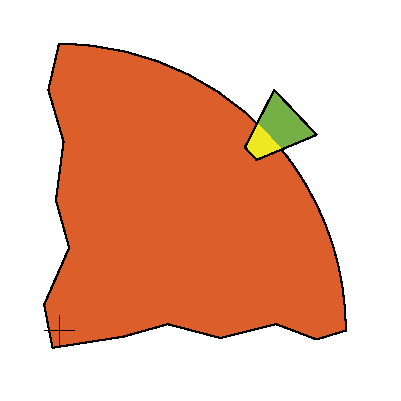
\includegraphics{uberlagerung}
	\caption{Hier ist die caption}
	\label{fig:uberlagerung}
\end{figure}

In Abbildung \ref{fig:uberlagerung} ist eine solche Überlagerungssituation dargestellt.
Das Werkzeug wird als grünes Polygon gezeigt, eine Schnittebene des Werkstücks als oranges Polygon.
Der Abstand der Polygoneckpunkte der Werkzeugschnitte ist dabei sehr niedrig gewählt um den Sehnenfehler zu minimieren.
Das erhöht in Folge die Rundheit des Polygons.

Die Sehne einer Raumkurve ist die gerade Verbindung von zwei Punkten entlang der Kurve.
Sie kann verwendet wreden, um den Verlauf der Raumkurve unbekannter mathematischer Entstehung geschickt anzunähern.
Ist die Raumkruve gekrümmt, existiert über den Verlauf der Sehne ein Abstand zwischen Kurve und Gerade.
Das Maximum dieses Abstands ist definiert als der Sehnenfehler und dieser kann verringert werden, wenn der Abstand der Punkte auf der Raumkurve verringert wird.

Zusätzlich wurde bei der Diskretisierung des Werkstückzylinders in Schnittebenen die Position der Eckpunkte abwechselnd um den halben Abstand der Sehnenpunkte verschoben.
Damit kann der mittlere Abstand der diskreten Punkte auf der Oberfläche des Zylinders verringert werden.
So entstehen bei der Vernutzung des Simulationsergebnisses auf der unbearbeiteten Oberfläche des Werkstückes nicht-rechteckige Dreiecke.
Diese Dreiecksform ist für die gängige Vernetzungsalgorithmen besser geeignet als rechteckig.

Es wurden keine Versuche angestellt die Rundheit der Schnittgeometrien zu berechnen und die Simulationsgenauigkeit in Abhängigkeit davon zu bewerten.
Auch gilt es noch zu untersuchen, welchen Einfluss die Anzahl Eckpunkte bei der Diskretisierung auf die Simulationsgeschwindigkeit hat, da dieser als gering vermutet wurde.

Die in Abbildung \ref{fig:uberlagerung} gelb dargestellte Fläche ist der Überlagerungsbereich von Werkzeug- und Werkstückoperation.
Dieser überlagerte Bereich wird bei der Simulation der Schnittoperation von dem Werkstückpolygon abgezogen.

\section{Plotten}
Die Architektur des Codes erlaubt das parallel zum Lösen des mathematischen Problems die Ausgabe erfolgt mit minimalem Einfluss auf die Ausführungsgeschwindigkeit der Berechnung.
Das wurde erreicht durch die Auslagern des Plottens in eine Klasse.
